\section{Method} \label{sec:method}

%Currently, the IEC Wave Resource Assessment technical specification (TS) focuses on quantifying resource parameters that are important to characterizing the resource across different spatial scales (i.e., three "classes" of resource assessment), but it provides little guidance on how to sum the theoretical resource for a region or site of interest. This is because this technical specification is focused primarily on characterizing the resource for feasibility studies (class 1 and 2) and quantifying the resource for designing projects where technologies are known (class 3). At the feasibility level, omni-directional wave power serves as a useful metric for quantifying the opportunity for wave energy development. When conducting array design, the TS states that ``the effects of the WEC array on wave propagation should be included in the numerical model. Any modifications made to the numerical model to account for the effects of a WEC array shall be documented and justified.'' This is important guidance that effectively accounts for wave directionality, but it is not practical or feasible when performing large-scale theoretical resource assessments for arbitrary devices. Instead, the approach used here skips the complexity of simulating many (thousands to millions or more?) of individual WECs extracting energy, and instead treats the line as a `perfect' array that extracts all of the incoming energy. By using a line-integral (dot-product), we are accounting for the directionality of waves (i.e., the `shadowing effect' of arrays) that is called for in the standards. Thus, the line-integral approach effectively accounting for the `shadowing effect' that is required by the IEC TS, and therefore this approach is consistent with it.


\begin{figure}[ht]
\centering
%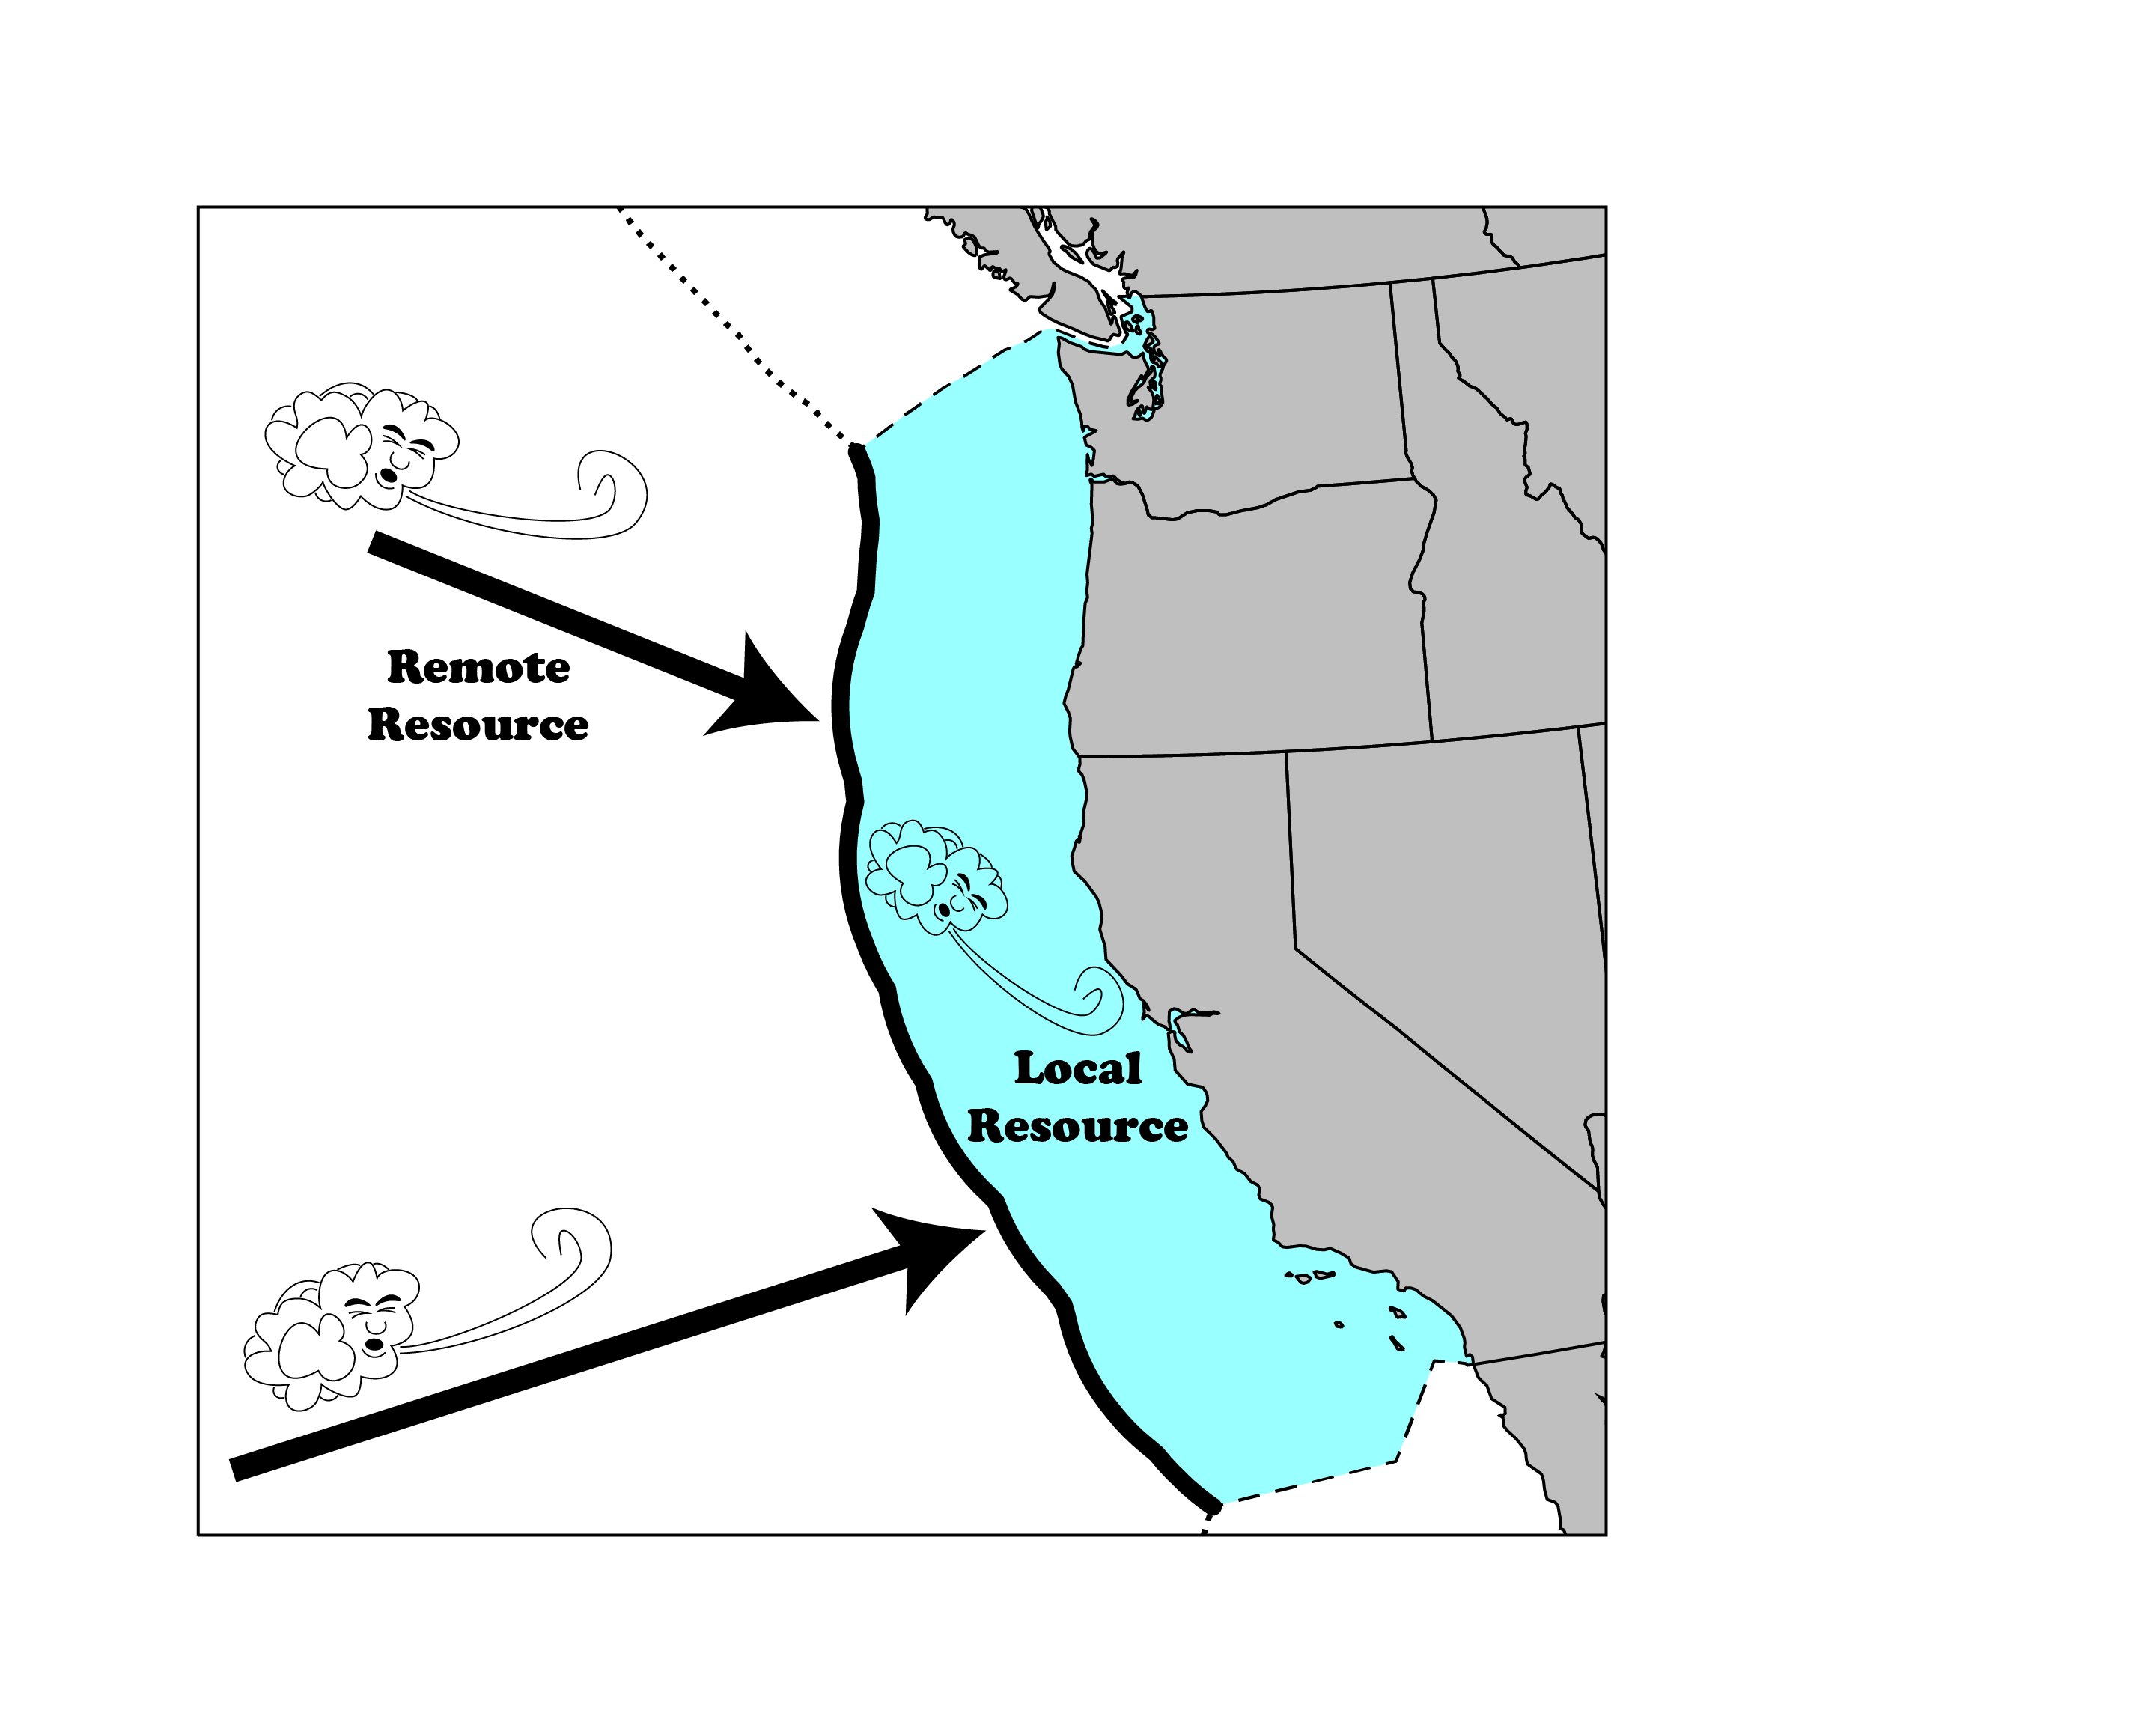
\includegraphics[width=0.9\linewidth]{../diagram/EEZ_contour03_edit01.png}
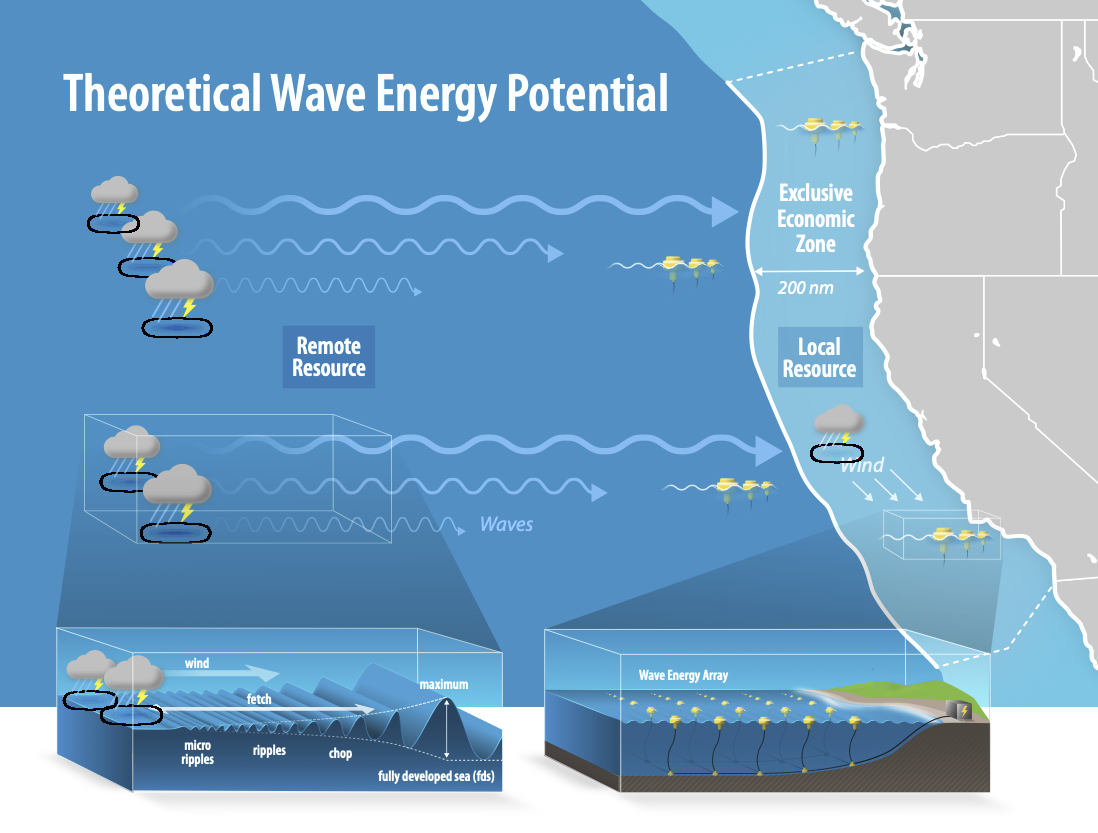
\includegraphics[width=\linewidth]{../fig/NREL-water-NatureEnergyGraphic-Levi-FY21-jfrenzl-v5.png}
%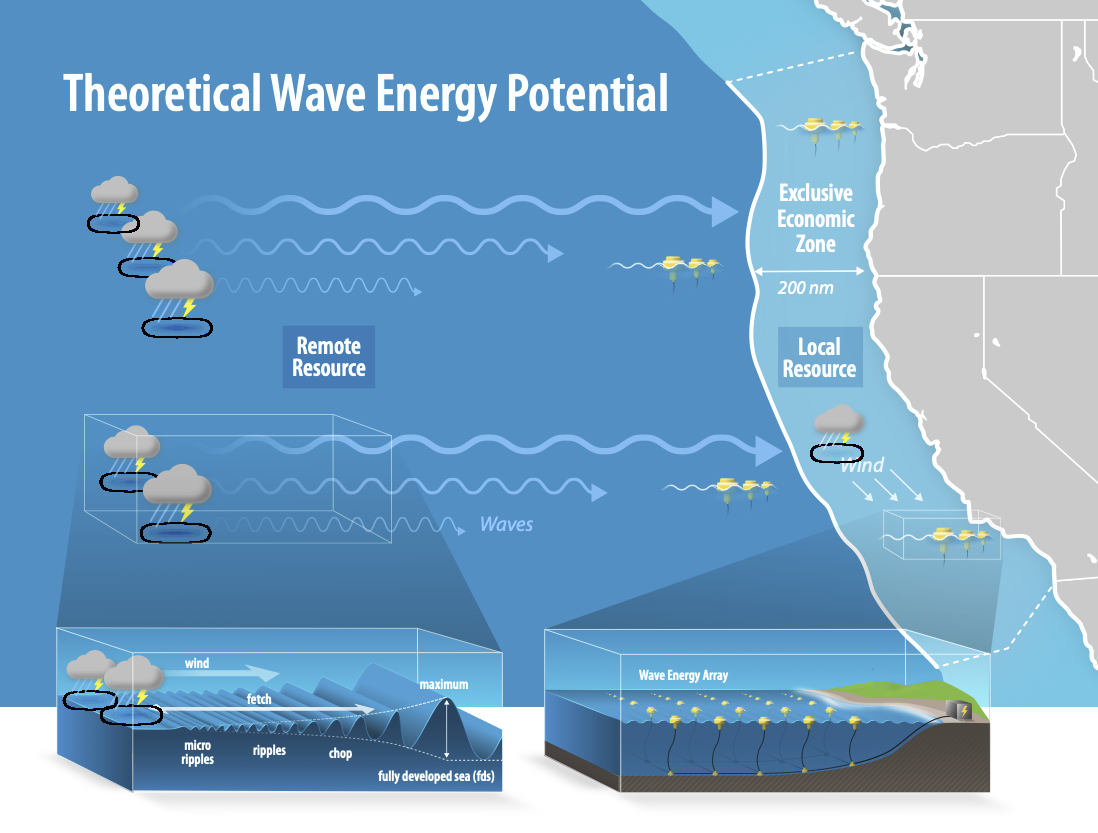
\includegraphics[width=\linewidth]{../fig/NREL-water-NatureEnergyGraphic-Levi-FY21-jfrenzl-v5.pdf}
\caption{A diagram depicting the U.S. West Coast's wave energy resource. Insets show the generation of waves by storms (left), and a schematic of a hypothetical wave array (right).}
\label{fig:diagram:west-eez}
\end{figure}

The proposed methodology eliminates ``double counting'' and includes all sources of wave energy that are legitimately a portion of the region's resource. Specifically,

\begin{enumerate}
    \item This methodology follows IEC TS-101 standards for numerical model setup, configuration, and validation. The IEC standards provide internationally accepted guidelines for model setup and procedures for validation. In addition to the IEC requirements, the model must also be configured to output the source terms, so that the `local resource' (defined below) can be computed.
    
    \item The total wave resource is defined as the sum of the remote and local resource (Figure \ref{fig:diagram:west-eez}). To our knowledge, this is the first work to define and propose including the local resource in the total resource estimate.
    
    The remote resource is defined as the wave energy that propagates into the domain. The remote resource is calculated utilizing a one-way dot-product at the boundary of the domain. This approach has been used in several previous wave resource assessments \citep{gunnQuantifyingGlobalWave2012, hemerRevisedAssessmentAustralia2017, regueroGlobalWavePower2015}.
    
     The inclusion of the local resource is a means for accounting for the `recovery' of the wave-field inshore of where energy is extracted. The local resource is the wave energy that is generated by winds within the boundary of the domain. Adding this local energy resource directly accounts for wave energy created by winds inshore of the chosen boundary. To the authors' knowledge this has not been considered in previous resource assessments.

    \item Extend the assessment to the edge of the region's legal boundaries. Based on Article 56 of the U.N. Law of the Sea — which states that ``in the exclusive economic zone, the coastal State has sovereign rights [to] the production of energy from the water, currents and winds'' — we propose that national resource assessments should utilize the exclusive economic zone (EEZ) as the domain over which wave energy resource totals are calculated (United Nations General Assembly 1982). \note{This isn't relavent for the inner-shelf resource. Do we need to revise this to say something like ``use consistent boundary definitions... we propose/use two: 1) EEZ, 2) 10 nmi, which provide `comprehensive' and `near-term/realistic' estimates, respectively.''}
\end{enumerate}

\subsection{Numerical Model} \label{sec:method:model}

Wave resource assessments use wave model `hindcasts' to estimate the history of the wave field over the region(s) of interest, and resource estimates are computed from the output of these models \citep{internationalelectrotechnicalcommissionPart101Wave2015}. This work uses WAVEWATCH III\textregistered v5.16 spanning a 31-year period from 1 January 1980 to 31 December 2010 \citep{tolmanDistributedmemoryConceptsWave2002,tolmanwavewatch}.

WAVEWATCH III\textregistered \ (hereafter WW3) is a well established numerical model that has been implemented successfully in many previous wave resource assessments \citep[e.g.,][]{garcia-medinaWaveResourceAssessment2014,hemerRevisedAssessmentAustralia2017,yangWaveModelTest2017}.
WW3 solves the five-dimensional action balance equation:

\begin{align}
  \frac{d N}{d t} = \frac{\Src{tot}}{\sigma} = \frac{1}{\sigma}\left ( \Src{in} + \Src{ds} + \Src{brk} + \Src{nl} + \Src{bot} \right )
  \label{eqn:actionbalance}
\end{align}
where $N(t,x,y,\sigma,\theta) \equiv D/\sigma$ is the wave action, $D$ is the variance spectrum, $t$ is time, $x$ and $y$ are the spatial coordinates, $\sigma$ is the radian frequency, and $\theta$ is the direction of wave propagation.
The wave action is conserved in the absence of sinks and sources of energy, their combined effect is represented as $\Src{tot}$. The model does not include the effects of wave reflection (e.g., at the shoreline), or of currents.

In this study we implement the ``ST4'' physics package option in WW3 to simulate wind energy input ($\Src{in}$) and dissipation due to whitecapping ($\Src{ds}$) \citep{ardhuinObservationSwellDissipation2009}.
The wind forcing is taken from NOAA's Climate Forecast System Reanalysis (CFSR) \citep{sahaNCEPClimateForecast2010}. The non-linear quadruplet interactions ($\Src{nl}$) are modeled with the Hasselmann and Hasselmann (\citeyear{hasselmannComputationsParameterizationsNonlinear1985}) formulation. Bottom friction ($\Src{bot}$) and depth induced wave breaking ($\Src{brk}$) are modeled with the JONSWAP Hasselmann etal. \citeyear{hasselmannMeasurementsWindwaveGrowth1973} and Battjes and Janssen \citeyear{battjesEnergyLossSetup1978} models, respectively. Finally, the effect of sea ice is considered by using a time varying mask based on the ice coverage fields from CFSR. Default parameters are used for all formulations. The wave spectrum is discretized with 24 equally spaced bins in $\theta$ space and 29 logarithmically spaced frequency bins from 0.035Hz to 0.5Hz with an increment factor of 1.1.

Model grids and bathymetry come from the NOAA NCEP hindcast Phase 1 mosaic-model \citep{chawla2011wavewatch,chawla201230}. In this system a global model (0.5$^{\circ}$ resolution) drives regional models (10" - 4" resolution) providing complete coverage over the U.S. EEZ with higher resolution focused on shallower waters. This model configuration is mostly aligned with the IEC TS 62600-101 requirements for a reconnaissance class resource assessment \citep{internationalelectrotechnicalcommissionPart101Wave2015}. \note{Why ``mostly''?}

The model was re-implemented to store directionally-resolved wave spectra and directionally-integrated source terms. These model outputs are collected along contours spaced 10 nmi apart (18.5 km) from shore to the EEZ boundary (200 nmi from shore). Data is saved at $1/6^\circ$ increments along each contour. This was done around Alaska (excluding the Arctic Coast), Atlantic Coast, Caribbean Coast (including Puerto Rico and U.S. Virgin Islands), Gulf Coast, Hawaii (excluding the Papah$\bar{\text{a}}$naumoku$\bar{\text{a}}$kea Marine National Monument), and the West Coast. 

\subsection{The Total Resource ($R_T$) \label{sec:method:calc}}

In this work we propose that the total theoretical wave resource, $R_T$, be defined as a sum of `remote' and `local' components:
\begin{align}
  R_T = R_R + R_L
\end{align}
The remote resource, $R_R$, is the piece of the wave energy resource that has previously been defined as the total wave resource \citep{gunnQuantifyingGlobalWave2012,EPRIwaveresource2011}.%, while the local resource, $R_L$, has not previously been included in wave resource assessments.

\subsubsection{Remote Resource} \label{sec:method:calc:remote}

The remote resource is computed as a line-integral of the wave energy that fluxes toward the coastline across the EEZ boundary when it is bordered by international waters. 

\begin{align}
  R_R = \rho g \int_{\ell}\iint \delta \, c_g(f) \, \bar{D}(f,\theta) \d f \d \theta \d l
\label{eqn:RR}
\end{align}
Where $c_g(f)$ is the wave group velocity, $\ell$ is the integration contour, and
the over-bar denotes a time-average of the wave-variance spectrum over the 31-year model period.

The directionality coefficient is $\delta = \cos(\theta_n - \theta)$ for waves propagating toward the coastline, and $\delta = 0$ otherwise.  $\theta_n$ is the direction normal to the contour pointing toward the shoreline. Utilizing this `one-way dot-product', is important because it minimizes the double counting found in `direction agnostic' approaches \citep[e.g., ][]{EPRIwaveresource2011}, and also does not erroneously subtract from the total where wave energy propagates offshore across the domain boundary \citep{nationalresearchcouncilEvaluationDepartmentEnergy2013,gunnQuantifyingGlobalWave2012}.

The integration contour $\ell$ is the segments of the U.S. EEZ that separate U.S. EEZ waters from the open-ocean (hereafter the `EEZ boundary'; thick black line in Figure \ref{fig:diagram:west-eez}), and does not include the EEZ segments that separate one nation's EEZ from that of a neighbor \citep[]{flandersmarineinstituteMaritimeBoundariesGeodatabase2018}. This is because wave-energy that fluxes across EEZ borders will be counted by the nation from which that resource originated, and should not be counted a second time where it fluxes across the border into a neighboring nation's EEZ.

\subsubsection{Local Resource} \label{sec:method:calc:local}

The local resource is computed as an area-integral of the following wave source- and sink-terms:

\begin{align}
  R_L &= \rho g \int_{EEZ}\iint \left ( \bar{S}_{in} + \bar{S}_{ds} + \bar{S}_{nl} \right ) \d \theta \d f \d A
\label{eqn:RL}
\end{align}
where $dA$ is differential-area. The frequency integral is taken over the range where waves are actively simulated in the model \citep[up to $0.5$ Hz,][]{ardhuinObservationSwellDissipation2009}. \note{Does this also apply to $R_R$?}

Note that the depth-induced wave breaking ($S_{brk}$) and bottom friction ($S_{bot}$) terms are neglected in \eqref{eqn:RL} because they close \eqref{eqn:actionbalance} by dissipating all of the energy that arrives at the shoreline. Including these terms, therefore, would be contrary to the purposes of resource assessment, because the goal is to calculate how much wave energy exists \textit{before} it dissipates at the shoreline.

It is tempting to also ignore the white-capping ($\bar{S}_{ds}$) and non-linear terms ($\bar{S}_{nl}$) — both of which are also negative across this frequency range — because this would yield a significantly larger estimate of $R_L$. Doing so, however, is scientifically questionable for three reasons. First, the spatial and temporal scales at which $S_{in}$ delivers energy to the wave field is similar to the scales at which $S_{ds}$ removes it. Second, the details of wave-generation is an active area of research, with large uncertainty associated with each term's magnitude, but there sum is relatively well constrained as demonstrated by the performance of wave models in general \citep[e.g.][]{ardhuin_semiempirical_2010,van_vledder_source_2016}. Third, there are practical challenges to generating electricity at-scale from the high-frequency (short wavelength) portion of the spectrum where most of $S_{in}$ energy exists. Therefore, it makes sense to include the $S_{nl}$ and $S_{ds}$ terms in order to properly quantify the degree to which low-frequency waves are generated by winds.

\subsection{The Inner-Shelf Resource ($R_I$)}

The approach above for provides a comprehensive and consistent methodology for assessing the total resource that is available to a nation. However, because the EEZ extends 200 nautical miles from shore — and given the pre-commercial state of wave energy technology — it is unrealistic to expect that all of this wave energy can be harnessed at large scale in the foreseeable future. For this reason, it is also useful to quantify the resource that is available closer to shore. We therefore also propose that it is useful to quantify the `inner-shelf resource', which we take to be the wave energy that is available within 10 nautical miles of shore.

The inner-shelf resource, $R_I$, is estimated according to \eqref{eqn:RR} with the integration contour, $\ell$, evaluated along the 10 nmi contour, rather than the EEZ boundary.  The local resource within 10 nmi of shore is small (5\% in Alaska, $<2$\% for all other regions), and so for simplicity we define $R_I$ only in terms of \eqref{eqn:RR}. This also suggests why most previous resource assessments may have neglected the local resource — because for the foreseeable future it is inaccessible.

\subsection{The Potential Resource ($R_P$)}

Because the source terms in \eqref{eqn:RL} depend on the sea-state and the sea-state depends on energy extracted ``up-wave'', there is ambiguity in estimating $R_L$ related to where and when wave energy is extracted by WECs. To address this, we calculate two estimates of $R_L$. The first, `natural local resource' ($R_L$) is calculated from the source-terms where waves from the global domain propagate freely throughout the EEZ. The second, `potential local resource' ($R_{L_*}$) is calculated from the source-terms when no wave energy propagates across the EEZ boundary. In other words, this is a `lake case' that only contains waves generated by winds within the regional domain. The potential resource is then defined as:

\begin{align}
    R_P = R_{L_*} - R_L
\end{align}

This `potential resource' is how much additional energy might be available in the local resource if the entirety of the remote resource, $R_R$, were extracted at the EEZ boundary. However, because accessing this energy is a long way from being technically viable we do not include it in $R_T$, and instead document it here as a way to indicate a maximum upper bound on wave energy potential.

\subsection{Summary}

There is an inherent tension throughout the field of resource assessment (i.e., beyond just wave energy) between including all possible sources, and being realistic about what is accessible. For this reason, the IEC — like other renewable energy sectors — has defined terminology that helps clarify some of the underlying assumptions that are made \citep[][]{internationalelectrotechnicalcommissionPartTerminologyEdition2020}. We propose that $R_T$ is the most appropriate estimate of a nation's theoretical resource, and that adding $R_P$ to this provides a maximum upper bound. While some might argue that some of the assumptions that go into these quantities are overly optimistic or pessimistic, we believe that this approach is as optimistic as possible without being unrealistic — which is exactly the intent of theoretical resource assessment.  On the other hand, for assessments of a nation's `technical' or `practical' resource, we suggest that — given the current state of wave energy technology — $R_I$ is the most appropriate quantity on which to base those assessments.

\subsection{Taken from discussion - is any of this needed?}

Including the natural or potential local resource in estimates of total theoretical wave energy assessments -- as we propose here -- is a fundamental change in methodology. There are several practical questions about how this energy can be harnessed on both large and small scales. 
The potential local resource only becomes available when large-scale wave energy extraction becomes economically feasible at great distance from shore. Even the natural local resource doesn't become a significant component of a wave energy project's resource until the size of the project is greater than several thousand square kilometers. As an example, consider fetch limited wave growth under a constant 10 m/s wind in deep water. Following \citet{donelan1980similarity} it will require 50 km of fetch for waves to have a modest wave flux of 1.5 kW/m. 

More work is needed to understand how much of the local resource overlaps with the offshore wind resource, and to identify what kinds of wave devices will efficiently harness the relatively high-frequency energy contained in the local resource. Though these questions and limitations exist, we still argue that including the local resource in the total theoretical resource is important for several reasons.
%\note{Z says: "we still argue" may be too weak? But I think it's the right tone?}

First, it is a real part of the total energy that is available -- or potentially available -- for conversion to electricity. Second, including it resolves outstanding questions associated with earlier resource assessments, thereby providing clarity to how regional wave resource assessments should be completed.  Third, including it broadens our understanding of what wave energy is; including it in our assessments gives a more complete picture of the opportunity. Fourth, and finally, the methodology proposed here -- which we have been applied at a regional scale -- can also be applied at the project scale to give an estimate of the theoretical resource at a site. This accuracy at all scales makes it ideally suited for broader adoption by the international community, which will in turn make the assessment of wave energy opportunities more comparable and transparent.

%%% Local Variables:
%%% TeX-master: "wave_res"
%%% End:
